\documentclass[11pt]{article}
\usepackage{amsmath, amssymb}
\usepackage{tikz}
\usepackage[paperwidth=12cm, paperheight=18cm, margin=1cm]{geometry}

\title{Five Equations That Changed the World}
\author{Typed live in vim}
\date{}

\begin{document}
\maketitle

\section{Euler's Identity}
The most beautiful equation in mathematics links five constants:
\[
  e^{i\pi} + 1 = 0
\]

\section{The Gaussian Integral}
\begin{align}
  \int_{-\infty}^{\infty} e^{-x^2}\,dx &= \sqrt{\pi} \\
  \frac{1}{\sigma\sqrt{2\pi}} \int_{-\infty}^{\infty}
    e^{-\frac{(x-\mu)^2}{2\sigma^2}}\,dx &= 1
\end{align}

\section{Maxwell's Equations}
\begin{align*}
  \nabla \cdot \mathbf{E} &= \frac{\rho}{\varepsilon_0} &
  \nabla \times \mathbf{E} &= -\frac{\partial \mathbf{B}}{\partial t} \\
  \nabla \cdot \mathbf{B} &= 0 &
  \nabla \times \mathbf{B} &= \mu_0 \mathbf{J}
    + \mu_0 \varepsilon_0 \frac{\partial \mathbf{E}}{\partial t}
\end{align*}

\section{Fourier Series}
\[
  f(x) = \frac{a_0}{2} + \sum_{n=1}^{\infty}
    \left( a_n \cos nx + b_n \sin nx \right)
\]
\begin{center}
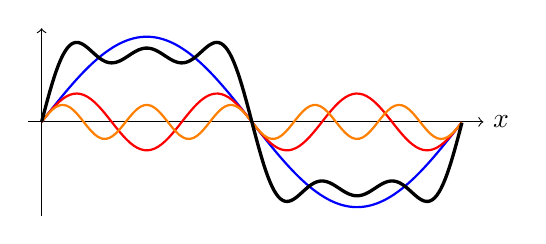
\begin{tikzpicture}[scale=0.85]
  \draw[->] (-0.2,0) -- (6.6,0) node[right] {$x$};
  \draw[->] (0,-1.4) -- (0,1.4);
  \foreach \n/\c in {1/blue, 3/red, 5/orange}
    \draw[\c, thick, domain=0:6.28, samples=120]
      plot (\x, {4/(pi*\n)*sin(\n*\x r)});
  \draw[black, very thick, domain=0:6.28, samples=200]
    plot (\x, {4/pi*(sin(\x r)+sin(3*\x r)/3+sin(5*\x r)/5)});
\end{tikzpicture}
\end{center}

\section{Bayes' Theorem}
\[
  P(A \mid B) = \frac{P(B \mid A)\, P(A)}{P(B)}
\]
\end{document}
